\documentclass[tikz,border=10pt]{standalone}
\usepackage[T1]{fontenc}
\usepackage[utf8]{inputenc}
\usepackage{lmodern}
\usepackage{amsmath,amssymb}
\usetikzlibrary{arrows.meta,positioning,shapes.geometric,calc}
\definecolor{jac}{HTML}{73539E}
\definecolor{ink}{HTML}{354052}
\tikzset{
 >=Stealth,
 state/.style={draw=jac,fill=jac!7,rounded corners=5pt,align=center,minimum width=26mm,minimum height=11mm,inner sep=5pt,font=\small},
 action/.style={state,fill=white},
 decision/.style={draw=jac,fill=jac!7,diamond,aspect=2.4,inner sep=1.8pt,align=center,font=\small},
 success/.style={state,draw=teal!75!black,fill=teal!7},
 failure/.style={state,draw=red!70!black,fill=red!5},
 arrow/.style={->,thick,draw=ink},
 note/.style={align=left,font=\footnotesize,text=ink}
}
\begin{document}

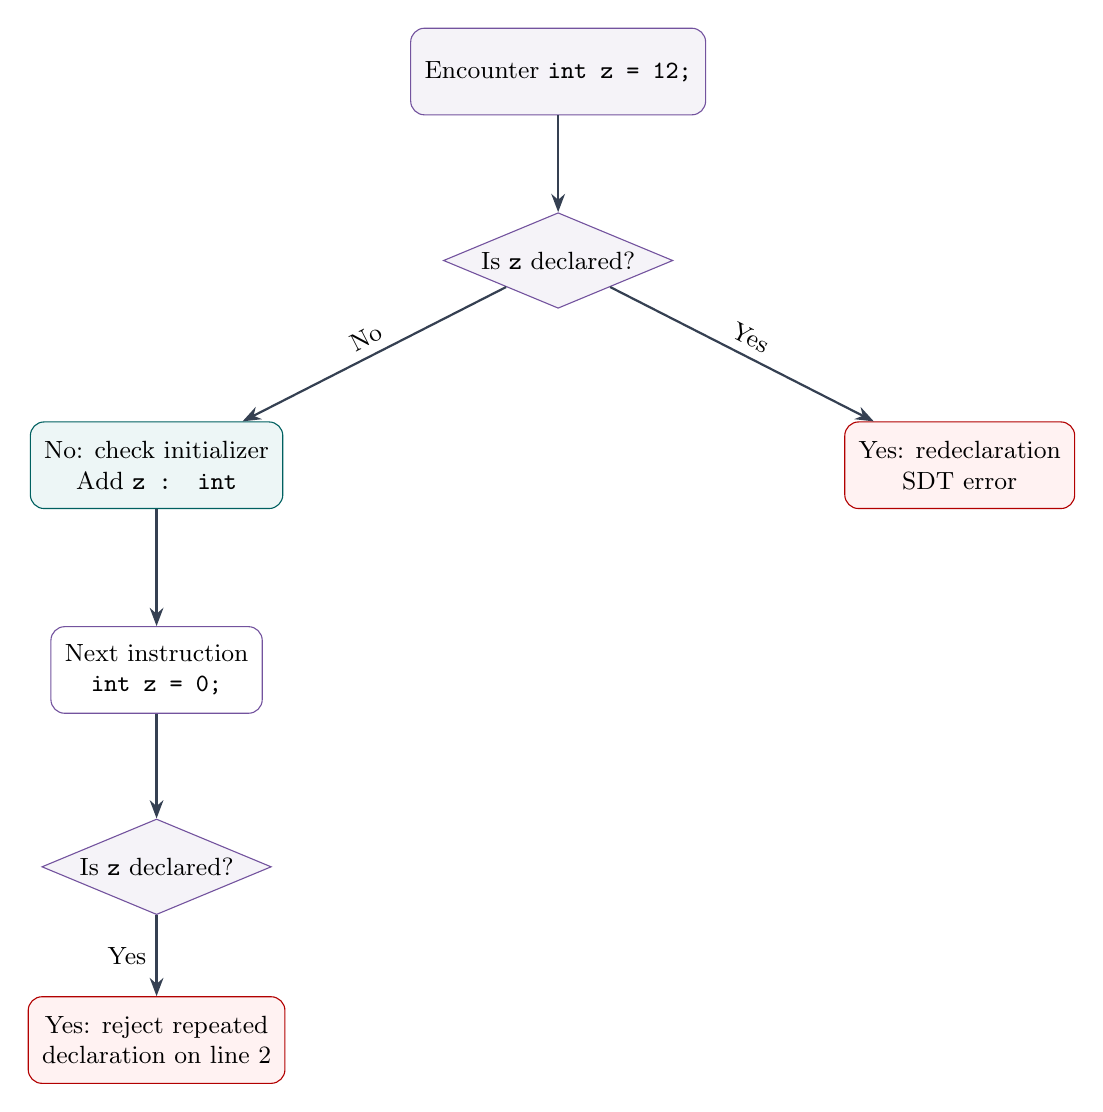
\begin{tikzpicture}[font=\small]
\node[state] (start) at (0,0) {Encounter \texttt{int z = 12;}};
\node[decision] (exists) at (0,-2.4) {Is \texttt{z} declared?};
\node[success] (new) at (-5.1,-5.0) {No: check initializer\\Add \texttt{z : int}};
\node[failure] (dup) at (5.1,-5.0) {Yes: redeclaration\\SDT error};
\node[action] (next) at (-5.1,-7.6) {Next instruction\\\texttt{int z = 0;}};
\node[decision] (again) at (-5.1,-10.1) {Is \texttt{z} declared?};
\node[failure] (err) at (-5.1,-12.3) {Yes: reject repeated\\declaration on line 2};
\draw[arrow] (start)--(exists);
\draw[arrow] (exists)--node[above,sloped]{No}(new);
\draw[arrow] (exists)--node[above,sloped]{Yes}(dup);
\draw[arrow] (new)--(next);
\draw[arrow] (next)--(again);
\draw[arrow] (again)--node[left]{Yes}(err);
\end{tikzpicture}

\end{document}
